\documentclass[10pt, a4paper]{article}


% ==> preamble
\usepackage{enumitem}
\usepackage{geometry}
\geometry{margin=0.1cm}
\pagestyle{empty}

\usepackage{tikz}
\usetikzlibrary{calc}


\def\mypic{
  \tikzpicture
  \clip (0,0) circle (2);
  \node at (0,-0.4) {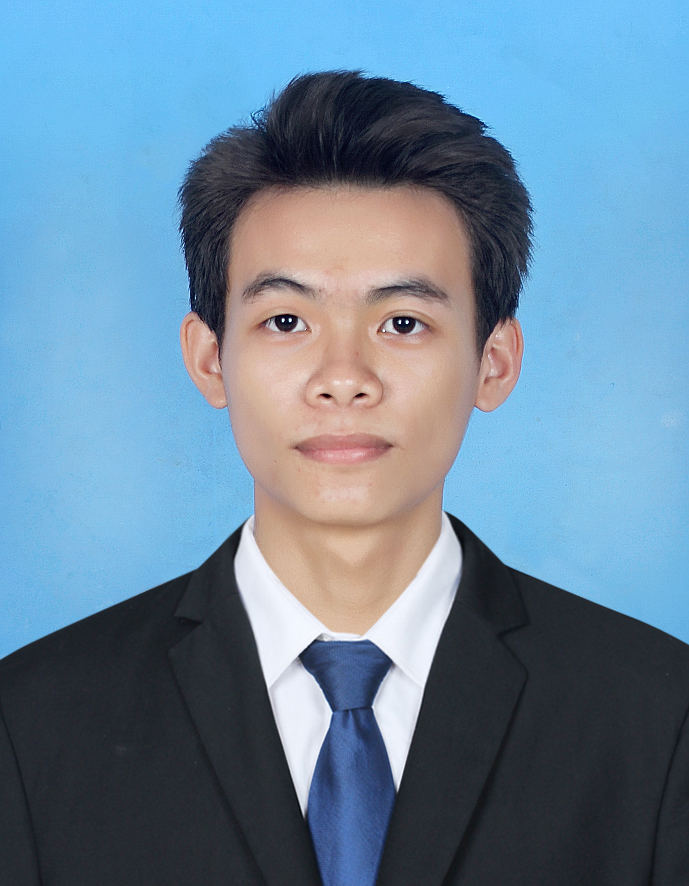
\includegraphics[scale=1.2]{me.jpg}};
  \endtikzpicture
}

\usepackage[no-math]{fontspec}
\setsansfont{Khmer OS Siemreap}[
	BoldFont = Khmer OS Bokor,
%	ItalicFont = Khmer OS Metal Chrieng,
	AutoFakeSlant=0.15,
	BoldItalicFont = Khmer OS Muol,
	Script=Khmer,Scale=1
]
\usepackage[Khmer, Latin]{ucharclasses}
\usepackage{etoolbox}
\XeTeXlinebreaklocale "khm"
\XeTeXlinebreakskip = 0pt plus 1pt minus 1pt

\newfontfamily{\khmerfamily}
[
	BoldFont = Kdam Thmor,
	ItalicFont = Khmer OS Metal Chrieng,
	BoldItalicFont = Khmer OS Muol,
	SmallCapsFont = TeX Gyre Pagella,
	Script=Khmer,Scale=1
]{Khmer OS Siemreap}
\newfontfamily{\englishfamily}{Fira Sans}[Ligatures=TeX, Scale=1.1] 
%Simonetta, Zeyada, Caveat, 
\newfontfamily{\monofamily}[Scale=1.25]{Latin Modern Mono}
\newfontfamily{\latinfamily}[Scale=1.3]{Latin Modern Roman}
\newfontfamily{\tacteingfamily}[Scale=3]{Tacteing}

% Define new font family (have to)   <-- BUG
\newrobustcmd{\englishfont}{\englishfamily\let\currentenglish\englishfamily }
\newrobustcmd{\khmerfont}{\khmerfamily\let\currentkhmer\khmerfamily}
\newrobustcmd{\mono}{\monofamily\let\currentenglish\monofamily }
\newrobustcmd{\en}{\latinfamily\let\currentenglish\latinfamily}
\newrobustcmd{\tacteing}{\tacteingfamily\let\currentenglish\tacteingfamily}



%% initialize the font
\khmerfont\englishfont
\setTransitionsForLatin{\currentenglish}{\currentkhmer}

% Change typewriter font family
\renewcommand{\ttfamily}{\mono}


\usepackage{bbold}
%\usepackage{fourier}
\let\altmathbb\mathbb
\AtBeginDocument{\let\mathbb\altmathbb}

% change math fonts
\let\temp\rmdefault
\usepackage{mathpazo}
\let\rmdefault\temp



\newcommand{\kml}
{
	\fontspec[
		Script=Khmer, Scale=1,
		AutoFakeBold=1, AutoFakeSlant=0.25
	] {Khmer OS Muol Light}
	\selectfont
}

\newcommand{\km}
{
	\fontspec[
		Script=Khmer, Scale=1,
		AutoFakeBold=1, AutoFakeSlant=0.25
	] {Khmer OS Muol}
	\selectfont
}

\newcommand{\kpali}
{
	\fontspec[
		Script=Khmer, Scale=1,
		AutoFakeBold=1, AutoFakeSlant=0.25
	] {Khmer OS Muol Pali}
	\selectfont
}

%create khmer counter
%khmer number
\makeatletter
\def\khmer#1{\expandafter\@khmer\csname c@#1\endcsname}
\def\@khmer#1{\expandafter\@@khmer\number#1\@nil}
\def\@@khmer#1{%
	\ifx#1\@nil% terminate when encounter @nil
	\else%
	\ifcase#1 ០\or ១\or ២\or ៣\or ៤\or ៥\or ៦\or ៧\or ៨\or ៩\fi%
	\expandafter\@@khmer% recursively map the following characters
	 \fi}
	 
% khmer alphabet
\def\khmernumeral#1{\@@khmer#1\@nil}
\def\alpkh#1{\expandafter\@alpkh\csname c@#1\endcsname}
\def\@alpkh#1{%
	\ifcase#1% zero -> none
	\or ក\or ខ\or គ\or ឃ\or ង%
	\or ច\or ឆ\or ជ\or ឈ\or ញ%
	\or ដ\or ឋ\or ឌ\or ឍ\or ណ%
	\or ត\or ថ\or ទ\or ធ\or ន%
	\or ប\or ផ\or ព\or ភ\or ម%
	\or យ\or រ\or ល\or វ\or ស%
	\or ហ\or ឡ\or អ%
	\else%[most]
	\@ctrerr % otherwise, counter error!
	\fi}
\makeatother


%% Khmer & math
\def\KHstop{\quad\text{។}}
\def\KHand{\quad\text{និង}\quad}
\def\KHor{\quad\text{ឬ}\quad}

\def\chaptername{ជំពូកទី}

\usepackage{fontawesome}
% <==
\def\mybold{\bfseries\large}
\linespread{1.2}
\usepackage{hyperref}
\hypersetup{
  colorlinks=true,
  linkcolor=magenta,
  filecolor=blue,      
  urlcolor=cyan,
  pdfinfo={
    title = {Sivmeng HUN's Resume},
    author= {Sivmeng HUN}
  },
}

\def\labelitemi{{\faCaretRight}}
\def\labelitemii{{\faCaretRight}}



\def\mytitle#1{
  {
    \tikzpicture
    \draw[draw=gray] (0,0)--(10.5,0);
    \node[rectangle, draw=gray!40, inner sep=0.3cm, right,
    fill=gray!30, font=\color{black}] at (0,0) 
    {\mybold #1};
    \endtikzpicture
  }
}
\begin{document}

\begin{tikzpicture}[remember picture, overlay]

  % ==> define coordinate
  \def\wx{8cm}
  \def\wy{6.4cm}
  \def\margin{1cm}
  \coordinate (A) at (current page.north west);
  \coordinate (B) at (current page.north east);
  \coordinate (C) at (current page.south east);
  \coordinate (D) at (current page.south west);

  \coordinate (E) at ($(current page.north west)+(\wx,0)$);
  \coordinate (F) at ($(current page.south west)+(\wx,0)$);
  \coordinate (G) at ($(current page.north west)+(0,-\wy)$);
  \coordinate (H) at ($(current page.north east)+(0,-\wy)$);
  % <==
  % ==> me and my name
  \draw[gray] (E)--(F);
  \node[scale=1.2] (mypic) at ($(A)+(\wx/2, -\wy/2)$) {\mypic};
  \node[xshift=\margin, yshift=-1cm, font=\huge, right] at (G) {HUN Sivmeng};
  %\node[yshift=-5cm, font=\bfseries\huge] at (mypic) {HUN Sivmeng};
  %\draw[help lines] (A)--(G)--(H)--(B)--cycle;
  % <==
  % ==> left side
  \node[
    rectangle, anchor=north west,
    text width=6cm, text badly ragged
    ] at ($(G)+(\margin, -3cm)$)
    {
      % ==> personal info
      {\mybold Personal Info}\\
      \begin{itemize}
        \item[\faHome] Phnom Penh, Cambodia
        \item[\faCalendar] 27 September, 2003
        \item[\faGraduationCap] RUPP, ~Maths, ~2\textsuperscript{nd} year
        \item[\faGlobe] Language
          \begin{itemize}
            \item Khmer (native)
            \item English (elementary)
          \end{itemize}
      \end{itemize}
      \vspace{1cm}
      % <==
      % ==> contact info
      {\mybold Contact}\\
      \begin{itemize}
        \item[\faEnvelope] {\href{email}{\ttfamily mengsivmeng@gmail.com}}
        \item[\faPhoneSquare] {\href{phone}{\ttfamily (+855) 31 749 5858}}
        \item[\faFacebookSquare] {\href{facebook}{\ttfamily fb.com/meng.sivmeng.er}}
        \item[\faPaperPlane] {\href{telegram}{\ttfamily t.me/meng\textunderscore sivmeng}} 
        \item[\faGithub] {\href{github}{\ttfamily github.com/mengistic}}
      \end{itemize}
      \vspace{1cm}
      % <==
      % ==> hobbies
      {\mybold Hobbies}\\
      \begin{itemize}
        \item Reading math books 
        \item watching lecture notes on Youtube
        \item Streaming movies
        \item Ricing Linux
        \item Hanging out with friends
      \end{itemize}
      % <==

    };
  % <==
  \node[
    rectangle, anchor=north west,
    text width=10.5cm, text badly ragged
    ] at ($(E)+(\margin, -1cm)$) {

      % ==> education and awards
      \mytitle{\faGraduationCap~~Education and Achievement}
      \begin{itemize}[label={}, leftmargin=0mm]
        % ==> 2017-2020
        \item {\bfseries 2017--2020}\\
          \begin{itemize}
            \item Entered Hun Sen Highschool of Kamchaymear
            \item Was a 5\textsuperscript{th} ranking candidate in 
              {\itshape Cambodian Outstanding Student Competition 
              (Grade 9)} for mathematics in national round 
            \item Won two gold medals from two distinct mathematical
              competitions (WMI and SASMO)
          \end{itemize}
          % <==
          % ==> 2020
        \item {\bfseries 2020}\\
          \begin{itemize}
            \item 
              Was trained for {\itshape International Mathematical Olympiad} 
              (IMO) at RUPP for 3 months
            \item Completed a level 9 English program 
              at {Pannasastra} University of Cambodia (PUC)
          \end{itemize}
          % <==
          % ==> 2021
        \item {\bfseries 2021}
          \begin{itemize}
            %\item Entered {\itshape Royal University of Phnom Penh} (RUPP)
              %majoring in Mathematics
            \item 1\textsuperscript{st} year at RUPP, Maths major
            %\item 1\textsuperscript{st} year at IFL, English major
            \item Attended a course in {\itshape Real Analysis}
            \item Attended a course in {\itshape Linear Algebra}
            \item Achieved an overall GPA of 3.91 (1\textsuperscript{st} year)
          \end{itemize}
          % <==
          % ==> 2022
        \item {\bfseries 2022--Now}
          \begin{itemize}
            \item 2\textsuperscript{nd} year at RUPP, Maths major
            \item Attended a course in {\itshape Number Theory}
            \item Was selected for a mentoring program in Mathematics by
              {\itshape Forum for Pushing the Boundary} (FPB)
            \item Was a selected candidate for 
            Mathematical Association of Cambodia (MAC) training program
          \end{itemize}
          % <==
      \end{itemize}
      \vspace{0.4cm}
      % <==
      % ==> skills
      \mytitle{\faWrench~~Experienced with}
      \begin{itemize}
        \item[\faSuperscript]
          {\bfseries Maths:}
          {Linear Algebra, Real Analysis, Abstract Algebra}
        \item[\faTerminal] 
          {\bfseries Programming (know some basics): } 
          { C, C++, Python, Javascript, LaTeX, Asymptote, Markdown, HTML, Bash}
        \item[\faStackOverflow]
          {\bfseries Technology: }
          {Linux, Vim, Emacs, Command line, Git}
      \end{itemize}
      \vspace{0.3cm}
      % <==
      % ==> ref
      \mytitle{\faPaperclip~~Reference}
      \begin{itemize}
        \item[\faUser] Professor \textit{SEAM Ngonn}, 
          \begin{itemize}
            \item Deputy Head of Department of Mathematics, RUPP
            \item Email: \href{prof-ngonn}{\ttfamily seamngonn@yahoo.fr}
            \item Contact: \href{prof-ngonn-phone}{\ttfamily (+855) 12 896 156}
          \end{itemize}
      \end{itemize}
      % <==

    };



\end{tikzpicture}


\end{document}
